% PLUM Verify (Algorithm 6) internal pipeline — grounded in src/signatures/plum/verify.rs
% header (Step 1 FS challenges; Step 2 sumcheck + Merkle openings; Step 3 STIR + residuosity),
% and the per-verify primitive counts (project CLAUDE.md / PLUM §4.2): 977 Griffin perms,
% 28 t-th power-residue symbol checks. Honestly marks the DEFERRED STIR proximity test.
% Compile: pdflatex plum_verify_pipeline.tex
\documentclass[border=4pt]{standalone}
\usepackage{tikz}
\usepackage{newtxtext,newtxmath}
\usetikzlibrary{positioning,arrows.meta,fit,backgrounds,calc}
\begin{document}
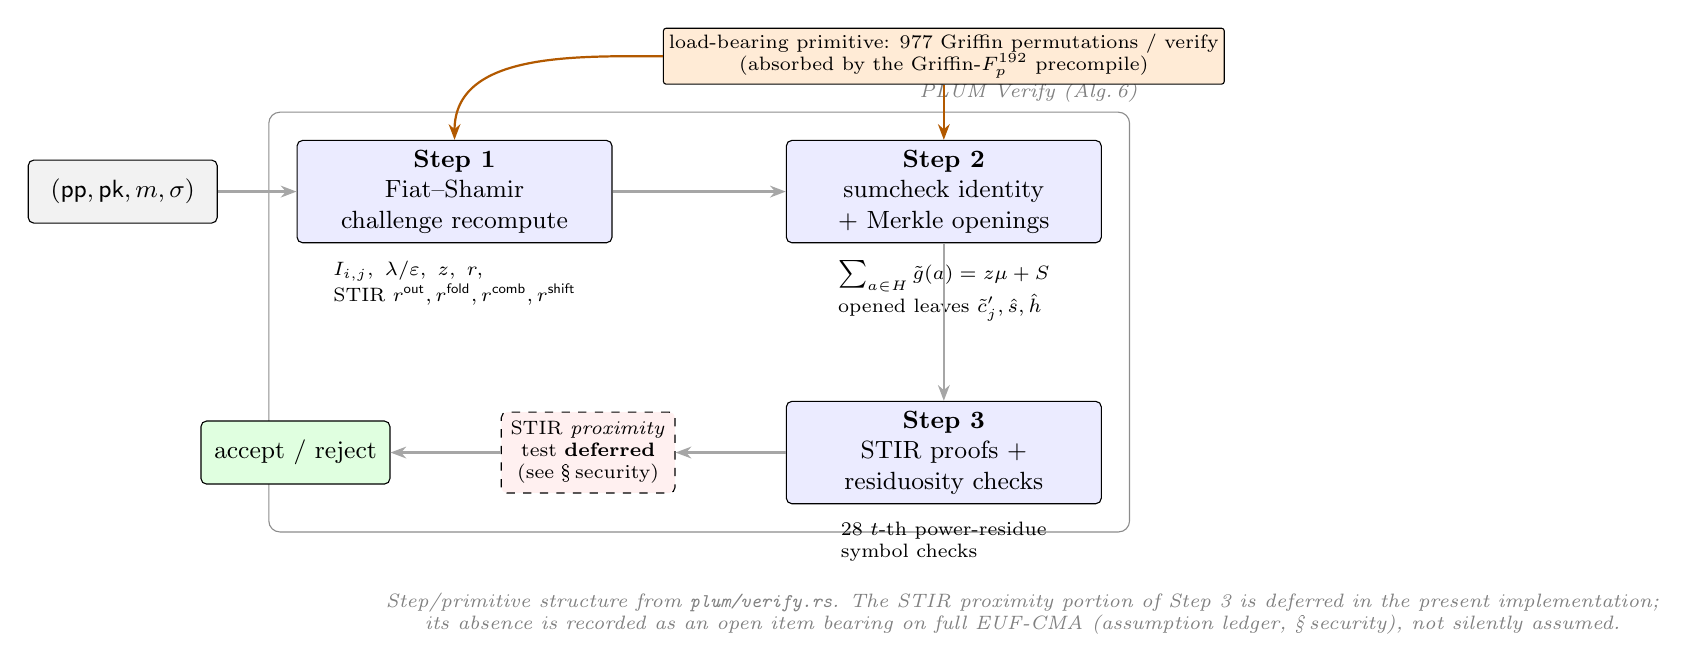
\begin{tikzpicture}[
  font=\small,>={Stealth[length=2mm]},
  io/.style={draw,rounded corners=2pt,fill=gray!10,minimum width=24mm,minimum height=8mm,align=center},
  phase/.style={draw,rounded corners=2pt,fill=blue!8,minimum width=40mm,minimum height=13mm,align=center},
  sub/.style={font=\scriptsize,align=left},
  prim/.style={draw,fill=orange!16,rounded corners=1pt,font=\scriptsize,inner sep=2pt,align=center},
  defer/.style={draw,dashed,fill=red!6,rounded corners=2pt,font=\scriptsize,align=center},
  lbl/.style={font=\scriptsize\itshape,gray},
  flow/.style={->,thick,gray!70},
]
% inputs
\node[io] (in) {$(\mathsf{pp},\mathsf{pk},m,\sigma)$};

% Step 1
\node[phase,right=10mm of in] (s1) {\textbf{Step 1}\\Fiat--Shamir\\challenge recompute};
\node[sub,below=1mm of s1] {$I_{i,j},\ \lambda/\varepsilon,\ z,\ r,$\\ STIR $r^{\mathsf{out}},r^{\mathsf{fold}},r^{\mathsf{comb}},r^{\mathsf{shift}}$};

% Step 2
\node[phase,right=22mm of s1] (s2) {\textbf{Step 2}\\sumcheck identity\\$+$ Merkle openings};
\node[sub,below=1mm of s2] {$\sum_{a\in H}\tilde g(a)=z\mu+S$\\opened leaves $\tilde c'_j,\hat s,\hat h$};

% Step 3
\node[phase,below=20mm of s2,fill=blue!8] (s3) {\textbf{Step 3}\\STIR proofs $+$\\residuosity checks};
\node[sub,below=1mm of s3] {$28$ $t$-th power-residue\\symbol checks};

% deferred box
\node[defer,left=14mm of s3] (def) {STIR \emph{proximity}\\test \textbf{deferred}\\(see \S\,security)};

% output
\node[io,left=14mm of def,fill=green!12] (out) {accept / reject};

% precompile-cost annotation
\node[prim,above=7mm of s2] (perm) {load-bearing primitive: $977$ Griffin permutations / verify\\(absorbed by the Griffin-$\mathbb{F}_p^{192}$ precompile)};

\draw[flow] (in) -- (s1);
\draw[flow] (s1) -- (s2);
\draw[flow] (s2) -- (s3);
\draw[flow] (s3) -- (def);
\draw[flow] (def) -- (out);
\draw[->,thick,orange!70!black] (perm) -- (s2);
\draw[->,thick,orange!70!black] (perm.west) to[out=180,in=90] (s1.north);

\begin{scope}[on background layer]
  \node[fit=(s1)(s2)(s3),draw=black!45,rounded corners,inner sep=10pt,
        label={[lbl]above right:PLUM Verify (Alg.\,6)}]{};
\end{scope}
\node[lbl,below=10mm of s3,align=center,xshift=10mm]
  {Step/primitive structure from \texttt{plum/verify.rs}. The STIR proximity portion of Step 3 is
   deferred in the present implementation;\\its absence is recorded as an open item bearing on
   full EUF-CMA (assumption ledger, \S\,security), not silently assumed.};
\end{tikzpicture}
\end{document}
